\documentclass[a4paper]{report}%imposto la classe la dimensione


\usepackage[T1]{fontenc} % codifica dei font per l'italiano
\usepackage[utf8]{inputenc} % lettere accentate da tastiera
\usepackage[italian]{babel} % lingua del documento
\usepackage[shortlabels]{enumitem}%per fare elenchi ad hoc
\usepackage{amsmath}% per avere le formule matematiche fatte bene
\usepackage{amssymb}% per avere le formule matematiche fatte bene
\usepackage{amsthm}%per fare i teoremi in modo ordinato
\usepackage[big]{layaureo} %per avere i margini più stretti
\usepackage[table]{xcolor}%per colorare le tabelle
\usepackage{framed}% per riquadrare il testo
\usepackage{calrsfs}% per avere le lettere calligrafiche
\usepackage{empheq} %per fare le equazioni per bene
\usepackage{titling}% per modificare il titolo
\usepackage{graphicx} %per inserire le immagini 
\usepackage{dirtytalk}% per mettere èiù facilmente le virgolette
\usepackage{titlesec}


%per mettere il sottotitolo
\newcommand{\subtitle}[1]{%
  \posttitle{%
    \par\end{center}
    \begin{center}\large#1\end{center}
    \vskip0.5em}%
}


%ridefinisco i set di numeri
\newcommand{\C}{\mathcal{C}}
\newcommand{\N}{\mathbb{N}}%naturali
\newcommand{\R}{\mathbb{R}}%reali
\newcommand{\prob}{\mathbb{P}} %probabilità
\newcommand{\Q}{\mathbb{Q}}%insieme Q


%ridefinisco alcune lettere greche per comodità
\renewcommand{\epsilon}{\varepsilon} %epsilon
\renewcommand{\theta}{\vartheta}%theta

%modifico i capitoli
\titleformat
{\chapter} % command
[display] % shape
{\normalfont\huge\bfseries} % format
{} % label
{0.5ex} % sep
{
    \vspace{1ex}
    \centering
} % before-code
[
\vspace{-0.5ex}%
] % after-code


\graphicspath{ {./images/} }


\begin{document}

%titolo
\title{Risposte ai Quesiti Teorici}
\subtitle{del corso di Analisi II del prof. Fabio Punzo}
\author{Jacopo Stringara}

\maketitle

%indice
\tableofcontents
\newpage

%fogli vari
\chapter{Foglio \ \thechapter}


\section*{Quesito 1}
\addcontentsline{toc}{section}{Quesito 1}
Dare le definizioni di: curva, equazioni parametriche di una curva, sostegno
di una curva, curva semplice, curva chiusa. Esibire: una curva semplice, una curva che
non è semplice, una curva chiusa, una curva che non è chiusa, due curve diverse con lo
stesso sostegno.

\medskip
\begin{large}
\textbf{Soluzione}
\end{large} \\
%==== Curva, Equazioni e Sostegno =====================================================
Si dice \textbf{Curva} un'applicazione continua $\varphi : I\subseteq \R\to\R^n$
e chiamiamo \textbf{Equazioni Parametriche} le equazioni:
\[
  t\in I \quad \varphi(t)=\left\{\begin{array}{l}
      x_1=\varphi_1(t)\\
      \vdots\\
      x_n=\varphi_n(t)
  \end{array}\right.  
\]
Inoltre definiamo \textbf{Sostegno} della Curva l'insieme $\varphi(I)\subseteq\R^n$\\
%==== Semplici, Chiusa =====================================================
Diremo che una Curva $\varphi: I\to\R^n$ è \textbf{Semplice} se:
\[
\forall t_1,t_2\in I \text{ con } t_1\neq t_2 \text{ (di cui uno interno) } \implies \varphi(t_1)\neq\varphi(t_2)  
\]
Una curva $\varphi:[a,b]\to\R^n$ invece si dice \textbf{Chiusa} se $\varphi(a)=\varphi(b)$.\\
%==== Esempi =================================================
\smallskip
\textbf{Esempi:}
\begin{align*}
  &\text{ Semplice: } \gamma(t)=(\cos t, \sin t)\: t\in[0,2\pi]\\
  &\text{ Non Semplice: } \gamma(t)=(\cos t, \sin t)\: t\in[0,4\pi]\\
  &\text{ Chiusa: } \gamma(t)=(\cos t, \sin t)\: t\in[0,2\pi]\\
  &\text{ Non Chiusa: } \gamma(t)=(t^2, t)\: t\in[0,1]\\
  &\text{ Curve diverse con stesso sostegno: } \gamma(t)=(\cos t, \sin t)\: t\in[0,2\pi] \text{ e }\gamma(t)=(\cos t, \sin t)\: t\in[0,4\pi]
\end{align*}


\section*{Quesito 2}
\addcontentsline{toc}{section}{Quesito 2}
Dare le definizioni di curva regolare, di curva regolare a tratti, di versore
tangente $T$. Esibire una curva di classe $C^1$
il cui sostegno abbia una cuspide.


\medskip
\begin{large}
\textbf{Soluzione}
\end{large}\\
Diremo che una Curva $\varphi : I = [a,b]\subseteq \R\to\R^n$ è \textbf{Regolare}
se:
\[
  \varphi\in C^1(I) \text{ e } \forall t \in (a,b) \quad \varphi'(t)\neq 0
\text{ (o equivalentemente } \|\varphi'(t)\|^2\neq0).
\]
Diremo invece che è \textbf{Regolare a Tratti}
se l'insieme I è divisibile in N ($\in\N$) tratti
in cui $\varphi$ è Regolare. Infine chiamiamo \textbf{Versore Tangente}
alla Curva nel punto $t_0$ il vettore:
\[
T(t_0)=\frac{\varphi'(t_0)}{\|\varphi'(t_0)\|}  
\]
Un esempio di Curva $C^1$ con Cuspide è il seguente:
\[
\varphi(t)=(t^3,t^2)\quad t\in[-1,1]
\]
Infatti si nota facilmente che $\varphi\in C^1([-1,1])$,
tuttavia non è Regolare in $0$ poichè $\varphi'(0)=(0,0)$. Se ne facciamo il grafico:
\begin{figure}[h]
  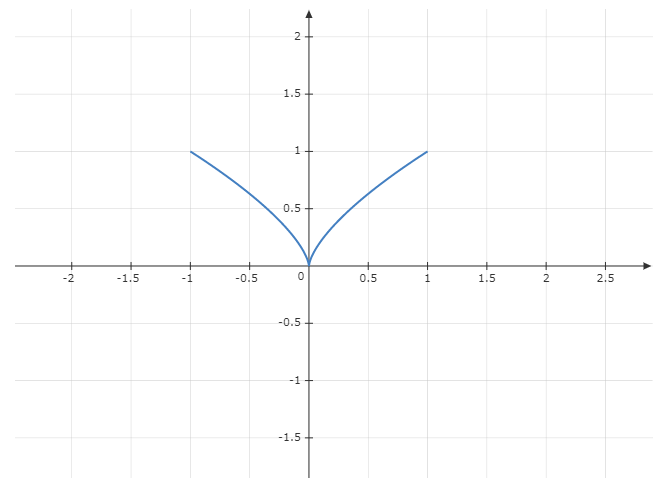
\includegraphics[width=\textwidth]{cuspide.png}
\end{figure}


\section*{Quesito 3}
\addcontentsline{toc}{section}{Quesito 3}
Dire cosa si intende per orientamento o verso di percorrenza di una curva.
Esibire due curve con lo stesso sostegno, ma con orientamento opposto. Dare la definizione
di curve equivalenti. Sotto quali condizioni sul cambiamento di parametro due curve
equivalenti hanno lo stesso orientamento o orientamento opposto?


\medskip
\begin{large}
\textbf{Soluzione}
\end{large}\\
Diremo che un punto $P_1=\varphi(t_1)$ di una Curva precede un altro punto $P_2=\varphi(t_2)$ se $t_1<t_2$.
Due curve con stesso sostegno ma orientamento opposto sono le seguenti:
\[
\varphi(t)=(\cos t, \sin t) \text{ e } \gamma(t)=(\sin t, \cos t) \text{ con } t\in [0,2\pi]  
\]
Diremo che due Curve $\varphi:I\to\R^n$ e $\gamma:J\to\R^n$ sono \textbf{Equivalenti} se:
\[
\exists \: g:I\to J \text{ suriettiva},\:C^1,\:g'(t)\neq0\;\forall t\in I \text{ tale che: } \varphi(t)=\gamma(g(t))
\]
E inoltre avranno lo stesso verso se $g'(t)>0$ e opposto se invece $g'(t)<0$
\section*{Quesito 4}
\addcontentsline{toc}{section}{Quesito 4}
Dare le definizioni di lunghezza di una curva e di curva rettificabile. Scrivere
la formula che fornisce la lunghezza di una curva di classe $C^1$.


\medskip
\begin{large}
\textbf{Soluzione}
\end{large}\\



\section*{Quesito 5}
\addcontentsline{toc}{section}{Quesito 5}
Cosa si intende per ascissa curvilinea (o parametro d’arco). Mostrare che data
una curva regolare si può sempre trovare una curva ad essa equivalente parametrizzata
con l’ascissa curvilinea.


\medskip
\begin{large}
\textbf{Soluzione}
\end{large}


\section*{Quesito 6}
\addcontentsline{toc}{section}{Quesito 6}
Scrivere la definizione di integrale curvilineo di prima specie. Dimostrare che
l’integrale curvilineo di prima specie è invariante per curve equivalenti. Dedurne che due
curve equivalenti hanno la stessa lunghezza.

\medskip
\begin{large}
\textbf{Soluzione}
\end{large}


\section*{Quesito 7}
\addcontentsline{toc}{section}{Quesito 7}
Sia $\varphi = \varphi(s)$ una curva con $s$ ascissa 
curvilinea. Dare la definizione di curvatura di $\varphi$ e 
spiegarne il significato geometrico. Quando $\varphi$ si dice 
biregolare? Riferendosi a $\varphi$, dare le definizioni di: 
versore normale principale $N(s)$, versore binormale $B(s)$.
Mostrare che $T(s)$, $N(s)$, $B(s)$ formano una base
 ortonormale di $\R ^3$
. Scrivere le definizioni
dei piani osculatore, normale, rettificante. Dire cosa si intende per cerchio osculatore e
per raggio di curvatura.


\medskip
\begin{large}
\textbf{Soluzione}
\end{large}


\section*{Quesito 8}
\addcontentsline{toc}{section}{Quesito 8}
Dare la definizione di curva piana. Sia $\varphi = \varphi(s)$ una
 curva con $s$ ascissa
curvilinea. Definire la torsione di $\varphi$ e illustrarne il 
significato geometrico. In che modo la
torsione e il versore binormale sono collegati al fatto che 
una curva è piana?

\medskip
\begin{large}
\textbf{Soluzione}
\end{large}


\section*{Quesito 9}
\addcontentsline{toc}{section}{Quesito 9}
Scrivere e dimostrare le formule di Frénet.

\medskip
\begin{large}
\textbf{Soluzione}
\end{large}


\section*{Quesito 10}
\addcontentsline{toc}{section}{Quesito 10}
Data una curva $\varphi = \varphi(t)$ con $t$ parametro qualsiasi, 
scrivere $T(t)$, $N(t)$, $B(t)$,
la curvatura $\kappa(t)$ e la torsione $\tau (t)$. Inoltre, 
scrivere e dimostrare la formula di decomposizione dell’accelerazione.

\medskip
\begin{large}
\textbf{Soluzione}
\end{large}

\chapter{Foglio \ \thechapter}


\section*{Quesito 1}
\addcontentsline{toc}{section}{Quesito 1}
Dire cosa si intende per equazione differenziale ordinaria lineare del primo
ordine. Scrivere la formula risolutiva e dimostrarla. Inoltre, scrivere la formula risolutiva
del problema di Cauchy associato e dimostrarla

\medskip
\begin{large}
\textbf{Soluzione}
\end{large}


\section*{Quesito 2}
\addcontentsline{toc}{section}{Quesito 2}
Dire cosa si intende per equazioni differenziale ordinaria lineare del secondo
ordine a coefficienti costanti omogenea. Qual è il polinomio caratteristico? Dire qual è
l’integrale generale e spiegare come si ricava.



\medskip
\begin{large}
\textbf{Soluzione}
\end{large}


\section*{Quesito 3}
\addcontentsline{toc}{section}{Quesito 3}
Qual è la struttura dell’integrale generale di una equazione differenziale ordinaria lineare del secondo ordine completa? Illustrare il metodo di somiglianza per la
determinazione di una soluzione particolare, nei casi in cui il termine noto è un polinomio
o una funzione esponenziale o una funzione trigonometrica.


\medskip
\begin{large}
\textbf{Soluzione}
\end{large}


\section*{Quesito 4}
\addcontentsline{toc}{section}{Quesito 4}
Dare le definizioni di: punto interno, punto esterno, punto di frontiera (o di
bordo), interno di un insieme, frontiera (o bordo), chiusura. Fornire esempi.


\medskip
\begin{large}
\textbf{Soluzione}
\end{large}


\section*{Quesito 5}
\addcontentsline{toc}{section}{Quesito 5}
Dire cosa si intende per insieme aperto, per insieme chiuso e per insieme
limitato. Caratterizzare gli insiemi aperti in termini del loro interno, e gli insiemi chiusi
in termini della loro chiusura. Fornire esempi.


\medskip
\begin{large}
\textbf{Soluzione}
\end{large}


\section*{Quesito 6}
\addcontentsline{toc}{section}{Quesito 6}
Dare la definizione di insieme compatto. Enunciare il teorema di Heine-Borel.
Dare la definizione di insiemi connesso e le definizioni equivalenti di insieme connesso per
archi e di insieme connesso per poligonali. Dare la definizione di insieme convesso. Fornire
esempi.

\medskip
\begin{large}
\textbf{Soluzione}
\end{large}


\section*{Quesito 7}
\addcontentsline{toc}{section}{Quesito 7}
Dire cosa si intende per insieme di definizione di una funzione di più variabili
$f(x_1, x_2, \dots , x_n)$ e per insieme di livello. Scrivere la definizione di limite.

\medskip
\begin{large}
\textbf{Soluzione}
\end{large}


\section*{Quesito 8}
\addcontentsline{toc}{section}{Quesito 8}
Spiegare come le restrizioni di una funzione $f(x, y)$ lungo successioni, grafici
di funzioni e curve permettono di dedurre la non esistenza del limite o di determinare un
candidato limite.

\medskip
\begin{large}
\textbf{Soluzione}
\end{large}


\section*{Quesito 9}
\addcontentsline{toc}{section}{Quesito 9}
Illustrare come si può utilizzare il teorema del confronto (o dei due carabinieri)
per il calcolo di limiti di funzioni di più variabili. Enunciare il criterio che permette il
1
calcolo di limiti per funzioni di due variabili tramite le coordinate polari. E’ vero che se
\[
f(x_0+\rho\cos \theta, y_0+\rho\sin\theta) \xrightarrow[\rho\to 0]{} L \quad \forall\theta\in [0,2\pi],   
\]
allora
\[
    \lim_{(x,y)\to(x_0,y_0)} f(x,y)=L \; ?
\]

\medskip
\begin{large}
\textbf{Soluzione}
\end{large}


\section*{Quesito 10}
\addcontentsline{toc}{section}{Quesito 10}
Dare la definizione di funzione di più variabili continua in un punto e di
funzione Lipschitziana in un sottoinsieme. Enunciare il teorema di Weierstrass e il teorema
di esistenza dei valori intermedi.

\medskip
\begin{large}
\textbf{Soluzione}
\end{large}

\chapter{Foglio \ \thechapter}


\section*{Quesito 1}
\addcontentsline{toc}{section}{Quesito 1}
Dare la definizione di derivate parziali, di funzione derivabile e di gradiente.
Può una funzione di due variabili essere derivabile in un punto $(x_0, y_0)$
 e non essere continua in $(x_0, y_0)$?

\medskip
\begin{large}
\textbf{Soluzione}
\end{large}


\section*{Quesito 2}
\addcontentsline{toc}{section}{Quesito 2}
Dare la definizione di derivata direzionale. In che modo le derivata parziali
sono collegate alle derivate direzionali? Può una funzione di due variabili essere derivabile
in un punto $(x_0, y_0)$ lungo ogni direzione e non essere continua in $(x_0, y_0)$?



\medskip
\begin{large}
\textbf{Soluzione}
\end{large}


\section*{Quesito 3}
\addcontentsline{toc}{section}{Quesito 3}
Dare la definizione di funzione differenziabile in un punto. Scrivere l’equazione
del piano tangente in un punto al grafico di una funzione di due variabili; sotto quale
ipotesi su $f$ esiste? Dimostrare che una funzione differenziabile in un punto $(x_0, y_0)$ è
continua e derivabile in $(x_0, y_0)$. Enunciare e dimostrare la formula del gradiente.


\medskip
\begin{large}
\textbf{Soluzione}
\end{large}


\section*{Quesito 4}
\addcontentsline{toc}{section}{Quesito 4}
Enunciare e dimostrare il teorema del differenziale totale.

\medskip
\begin{large}
\textbf{Soluzione}
\end{large}


\section*{Quesito 5}
\addcontentsline{toc}{section}{Quesito 5}
Enunciare e dimostrare il teorema sulle direzioni di massima e di minima
crescita.

\medskip
\begin{large}
\textbf{Soluzione}
\end{large}


\section*{Quesito 6}
\addcontentsline{toc}{section}{Quesito 6}
Enunciare il teorema di derivazione di funzioni composte. Dimostrare che il
gradiente di una funzione di due variabili è ortogonale alle curve di livello.

\medskip
\begin{large}
\textbf{Soluzione}
\end{large}


\section*{Quesito 7}
\addcontentsline{toc}{section}{Quesito 7}
Definire le derivate parziali seconde e la matrice Hessiana. Esibire una funzione
per cui $f_{xy}(x_0,y_0)\neq f_{yx}(x_0,y_0)$, per qualche $(x_0, y_0)$.

\medskip
\begin{large}
\textbf{Soluzione}
\end{large}


\section*{Quesito 8}
\addcontentsline{toc}{section}{Quesito 8}
Enunciare il teorema di Schwarz. Sotto quale ipotesi su $f$ la matrice Hessiana
è simmetrica?

\medskip
\begin{large}
\textbf{Soluzione}
\end{large}


\section*{Quesito 9}
\addcontentsline{toc}{section}{Quesito 9}
Enunciare e dimostrare il teorema di Lagrange e la formula di Taylor con resto
di Lagrange per funzioni di più variabili.


\medskip
\begin{large}
\textbf{Soluzione}
\end{large}


\section*{Quesito 10}
\addcontentsline{toc}{section}{Quesito 10}
Enunciare e dimostrare la formula di Taylor con resto di Peano.

\medskip
\begin{large}
\textbf{Soluzione}
\end{large}

\chapter{Foglio \ \thechapter}


\section*{Quesito 1}
\addcontentsline{toc}{section}{Quesito 1}
Dare la definizione di funzione $k$ volte differenziabile in un punto. Sotto quali
ipotesi su $f$, vale la formula di Taylor di ordine $k$ (cioè $f$ è $k$ volte differenziabile)?


\medskip
\begin{large}
\textbf{Soluzione}
\end{large}


\section*{Quesito 2}
\addcontentsline{toc}{section}{Quesito 2}
Cosa si intende per matrice Jacobiana di una funzione 
$f : A \subseteq \R^n \to \R^m$ ?
Scrivere la formula sulla matrice Jacobiana di funzione composta.


\medskip
\begin{large}
\textbf{Soluzione}
\end{large}


\section*{Quesito 3}
\addcontentsline{toc}{section}{Quesito 3}
Dare le definizioni di punto: di minimo relativo, di massimo relativo, di sella,
critico o stazionario. Enunciare e dimostrare il teorema di Fermat.


\medskip
\begin{large}
\textbf{Soluzione}
\end{large}


\section*{Quesito 4}
\addcontentsline{toc}{section}{Quesito 4}
Enunciare e dimostrare il criterio della matrice Hessiana per la classificazione
di punti critici.


\medskip
\begin{large}
\textbf{Soluzione}
\end{large}


\section*{Quesito 5}
\addcontentsline{toc}{section}{Quesito 5}
Enunciare e dimostrare la condizione necessaria perché un punto sia di massimo o di minimo relativo.

\medskip
\begin{large}
\textbf{Soluzione}
\end{large}


\section*{Quesito 6}
\addcontentsline{toc}{section}{Quesito 6}
Illustrare, anche mediante degli esempi, come si procede per classificare un
punto critico quando la matrice Hessiana nel punto è semidefinita negativa o positiva.

\medskip
\begin{large}
\textbf{Soluzione}
\end{large}


\section*{Quesito 7}
\addcontentsline{toc}{section}{Quesito 7}
Enunciare e dimostrare il teorema del Dini

\medskip
\begin{large}
\textbf{Soluzione}
\end{large}


\section*{Quesito 8}
\addcontentsline{toc}{section}{Quesito 8}
Enunciare il teorema del Dini nel caso in cui $F(x_0,y_0)=0, \: F_x(x_0,y_0)\neq 0$

\medskip
\begin{large}
\textbf{Soluzione}
\end{large}


\section*{Quesito 9}
\addcontentsline{toc}{section}{Quesito 9}
Enunciare e dimostrare la versione globale del teorema della funzione implicita.

\medskip
\begin{large}
\textbf{Soluzione}
\end{large}


\section*{Quesito 10}
\addcontentsline{toc}{section}{Quesito 10}
Sotto quali ipotesi su $F$, la funzione definita implicitamente $f$ è di classe $C^k$?
Nel caso esista, come si trova $f''(x)$?

\medskip
\begin{large}
\textbf{Soluzione}
\end{large}

\chapter{Foglio \ \thechapter}


\section*{Quesito 1}
\addcontentsline{toc}{section}{Quesito 1}
Enunciare il teorema del Dini nel caso in cui $F:A\subseteq \R^{n+1}\to\R$.

\medskip
\begin{large}
\textbf{Soluzione}
\end{large}


\section*{Quesito 2}
\addcontentsline{toc}{section}{Quesito 2}
Enunciare il teorema del Dini nel caso in cui $F:A\subseteq \R^{n+h}\to\R^h$.


\medskip
\begin{large}
\textbf{Soluzione}
\end{large}


\section*{Quesito 3}
\addcontentsline{toc}{section}{Quesito 3}
Mostrare che, applicando il teorema precedente in un intorno di un punto $P_0$
ad una funzione $F:A\subseteq \R^3\to\R^2$, si vede che l’insieme degli zeri di
$F$ in un intorno di $P_0$ è il sostegno di una curva regolare, semplice. Ricavare un vettore parallelo al vettore
tangente alla curva nel punto.


\medskip
\begin{large}
\textbf{Soluzione}
\end{large}


\section*{Quesito 4}
\addcontentsline{toc}{section}{Quesito 4}
Illustrare come si studia il grafico di una funzione $y = f(x)$ definita implicitamente globalmente da una equazione del tipo $F(x, y) = 0$.


\medskip
\begin{large}
\textbf{Soluzione}
\end{large}


\section*{Quesito 5}
\addcontentsline{toc}{section}{Quesito 5}
Utilizzando il teorema del Dini, dimostrare che $\nabla F$ è ortogonale all’insieme
degli zeri di una funzione $F(x, y)$. Come si ottiene lo stesso risultato nel caso di un insieme
di livello generale?


\medskip
\begin{large}
\textbf{Soluzione}
\end{large}


\section*{Quesito 6}
\addcontentsline{toc}{section}{Quesito 6}
Dire cosa si intende per vincolo di uguaglianza. Dare le definizioni di: punto
di minimo vincolato, punto di massimo vincolato, punto di estremo vincolato, punto di
minimo relativo vincolato, punto di massimo relativo vincolato, punto di estremo relativo
vincolato.


\medskip
\begin{large}
\textbf{Soluzione}
\end{large}


\section*{Quesito 7}
\addcontentsline{toc}{section}{Quesito 7}
Cosa si intende per derivata tangenziale al vincolo? Dare la definizione per
punto critico (o singolare) vincolato.

\medskip
\begin{large}
\textbf{Soluzione}
\end{large}


\section*{Quesito 8}
\addcontentsline{toc}{section}{Quesito 8}
Illustrare come si determinano punti di massimo e di minimo vincolati nel
caso di vincolo esplicitabile tramite il sostegno di una curva o l’unione di un numero finito
di grafici di funzioni di una variabile.


\medskip
\begin{large}
\textbf{Soluzione}
\end{large}


\section*{Quesito 9}
\addcontentsline{toc}{section}{Quesito 9}
Dare le definizioni di punto regolare e di punto singolare di un vincolo. Come
si definisce la Lagrangiana? Enunciare e dimostrare il teorema dei moltiplicatori di Lagrange. Quale parte del teorema dei moltiplicatori di Lagrange può essere vista come una
versione vincolata del teorema di Fermat?


\medskip
\begin{large}
\textbf{Soluzione}
\end{large}


\section*{Quesito 10}
\addcontentsline{toc}{section}{Quesito 10}
Illustrare come si determinano i punti di minimo e di massimo assoluto di
una funzione $f(x, y)$ continua in un insieme compatto $K\subseteq\R^2$.

\medskip
\begin{large}
\textbf{Soluzione}
\end{large}

\chapter{Foglio \ \thechapter}


\section*{Quesito 1}
\addcontentsline{toc}{section}{Quesito 1}
Dare le definizioni di misura interna ed esterna di un insieme limitato di $\R^n$,
di insieme misurabile secondo Peano-Jordan e di misura di un insieme.

\medskip
\begin{large}
\textbf{Soluzione}
\end{large}


\section*{Quesito 2}
\addcontentsline{toc}{section}{Quesito 2}
Esibire delle classi di insiemi misurabili in $\R^2$ e in $\R^3$.

\medskip
\begin{large}
\textbf{Soluzione}
\end{large}


\section*{Quesito 3}
\addcontentsline{toc}{section}{Quesito 3}
Esibire, motivando la risposta, un insieme di $\R^2$ non misurabile secondo PeanoJordan.

\medskip
\begin{large}
\textbf{Soluzione}
\end{large}


\section*{Quesito 4}
\addcontentsline{toc}{section}{Quesito 4}
Dare le definizioni di somme inferiori e superiori di Riemann, di funzione integrabile secondo Riemann e di integrale di Riemann. Quale classe di funzioni è integrabile
secondo Riemann su insiemi compatti misurabili?

\medskip
\begin{large}
\textbf{Soluzione}
\end{large}


\section*{Quesito 5}
\addcontentsline{toc}{section}{Quesito 5}
Scrivere le formule di riduzione (o di Fubini-Tonelli) per integrali doppi. Dare
una giustificazione approssimativa della formula.

\medskip
\begin{large}
\textbf{Soluzione}
\end{large}


\section*{Quesito 6}
\addcontentsline{toc}{section}{Quesito 6}
Dare le definizioni di dominio normale regolare e di dominio regolare. Scrivere
il teorema sulla formula di cambiamento di coordinate negli integrali doppi. Spiegare come
va intesa l’ipotesi $\phi$ di classe $C^1$
sul dominio regolare $\Omega '$, che è chiuso.

\medskip
\begin{large}
\textbf{Soluzione}
\end{large}


\section*{Quesito 7}
\addcontentsline{toc}{section}{Quesito 7}
Perché non si può applicare il teorema del Quesito 6 per ricavare il passaggio
da coordinate cartesiane a polari negli integrali doppi? Quale estensione del precedente
teorema permette di ottenere tale cambio di coordinate? Motivare le risposte.

\medskip
\begin{large}
\textbf{Soluzione}
\end{large}


\section*{Quesito 8}
\addcontentsline{toc}{section}{Quesito 8}
Scrivere le formule di integrazione per fili e per strati negli integrali tripli.
Dare una giustificazione approssimativa della formula.

\medskip
\begin{large}
\textbf{Soluzione}
\end{large}


\section*{Quesito 9}
\addcontentsline{toc}{section}{Quesito 9}
Enunciare e dimostrare il teorema di Pappo-Guldino.

\medskip
\begin{large}
\textbf{Soluzione}
\end{large}


\section*{Quesito 10}
\addcontentsline{toc}{section}{Quesito 10}
Spiegare come si definiscono gli integrali impropri (o generalizzati) in $\R^n$,
considerando il segno della funzione. Calcolare l’integrale della Gaussiana.

\medskip
\begin{large}
\textbf{Soluzione}
\end{large}

\chapter{Foglio \ \thechapter}


\section*{Quesito 1}
\addcontentsline{toc}{section}{Quesito 1}
Dare le definizioni di forma differenziale e di campo vettoriale.

\medskip
\begin{large}
\textbf{Soluzione}
\end{large}


\section*{Quesito 2}
\addcontentsline{toc}{section}{Quesito 2}
Come si definisce l’integrale curvilineo di seconda specie di una forma differenziale? E quello di un campo vettoriale?


\medskip
\begin{large}
\textbf{Soluzione}
\end{large}


\section*{Quesito 3}
\addcontentsline{toc}{section}{Quesito 3}
L’integrale curvilineo di seconda specie di una forma differenziale su due curve
equivalenti cambia? Motivare la risposta.


\medskip
\begin{large}
\textbf{Soluzione}
\end{large}


\section*{Quesito 4}
\addcontentsline{toc}{section}{Quesito 4}
Dare la definizione di forma differenziale esatta e di campo vettoriale conservativo. Cosa si intende per primitiva di una forma differenziale e per potenziale di un
campo vettoriale?

\medskip
\begin{large}
\textbf{Soluzione}
\end{large}


\section*{Quesito 5}
\addcontentsline{toc}{section}{Quesito 5}
Come si calcola l’integrale curvilineo di seconda specie di una forma differenziale esatta o di un campo vettoriale conservativo?

\medskip
\begin{large}
\textbf{Soluzione}
\end{large}


\section*{Quesito 6}
\addcontentsline{toc}{section}{Quesito 6}
Quanto vale l’integrale curvilineo di seconda specie di una forma differenziale
esatta lungo una curva chiusa? Motivare la risposta. Come si riformula lo stesso risultato
per i campi vettoriali conservativi?

\medskip
\begin{large}
\textbf{Soluzione}
\end{large}


\section*{Quesito 7}
\addcontentsline{toc}{section}{Quesito 7}
Enunciare e dimostrare il teorema sulla caratterizzazione delle forme differenziali esatte.

\medskip
\begin{large}
\textbf{Soluzione}
\end{large}


\section*{Quesito 8}
\addcontentsline{toc}{section}{Quesito 8}
Dare la definizione di forma differenziale chiusa e di campo vettoriale irrotazionale.

\medskip
\begin{large}
\textbf{Soluzione}
\end{large}


\section*{Quesito 9}
\addcontentsline{toc}{section}{Quesito 9}
Dimostrare che una forma differenziale esatta è anche chiusa.

\medskip
\begin{large}
\textbf{Soluzione}
\end{large}


\section*{Quesito 10}
\addcontentsline{toc}{section}{Quesito 10}
Esibire una forma differenziale chiusa che non sia esatta.

\medskip
\begin{large}
\textbf{Soluzione}
\end{large}

\chapter{Foglio \ \thechapter}


\section*{Quesito 1}
\addcontentsline{toc}{section}{Quesito 1}
Dare la definizione di insieme semplicemente connesso. Fornire esempi di
insiemi di insiemi semplicemente connessi e di insiemi non semplicemente connessi, in $\R^2$ e in $\R^3$.

\medskip
\begin{large}
\textbf{Soluzione}
\end{large}


\section*{Quesito 2}
\addcontentsline{toc}{section}{Quesito 2}
Dare le definizioni di insieme convesso e di insieme stellato rispetto a un
punto. In che relazione sono con gli insiemi semplicemente connessi? Fornire un esempio
di insiemi semplicemente connesso che non sia convesso e un altro che non sia stellato.

\medskip
\begin{large}
\textbf{Soluzione}
\end{large}


\section*{Quesito 3}
\addcontentsline{toc}{section}{Quesito 3}
Sotto quale ipotesi sull’insieme $A$, una forma differenziale chiusa in $A$ (un
campo vettoriale irrotazionale) è anche esatta in $A$ (conservativo)? Che succede se si
elimina tale ipotesi su $A$?

\medskip
\begin{large}
\textbf{Soluzione}
\end{large}


\section*{Quesito 4}
\addcontentsline{toc}{section}{Quesito 4}
Come si può rappresentare il bordo di un dominio regolare di $\R^2$ ? Sul bordo
sono ben definiti i versori tangente e normale?

\medskip
\begin{large}
\textbf{Soluzione}
\end{large}


\section*{Quesito 5}
\addcontentsline{toc}{section}{Quesito 5}
Cosa si intende per orientazione positiva della frontiera di un dominio regolare
di $\R^2$ ? E’ corretto dire che coincide con la frontiera percorsa in verso antiorario? Motivare
la risposta con degli esempi.

\medskip
\begin{large}
\textbf{Soluzione}
\end{large}


\section*{Quesito 6}
\addcontentsline{toc}{section}{Quesito 6}
Enunciare e dimostrare le formule di Gauss-Green in domini normali regolari
rispetto all’asse $x$ o rispetto all’asse $y$.

\medskip
\begin{large}
\textbf{Soluzione}
\end{large}


\section*{Quesito 7}
\addcontentsline{toc}{section}{Quesito 7}
Dedurre le formule di Gauss-Green in domini regolari che sono normali sia
rispetto all’asse $x$ che all’asse $y$.


\medskip
\begin{large}
\textbf{Soluzione}
\end{large}


\section*{Quesito 8}
\addcontentsline{toc}{section}{Quesito 8}
Enunciare le formule di Gauss-Green in domini regolari.

\medskip
\begin{large}
\textbf{Soluzione}
\end{large}


\section*{Quesito 9}
\addcontentsline{toc}{section}{Quesito 9}
Scrivere e dimostrare le formule che permettono di calcolare l’area di una
regione piana mediante le formule di Gauss-Green.

\medskip
\begin{large}
\textbf{Soluzione}
\end{large}


\section*{Quesito 10}
\addcontentsline{toc}{section}{Quesito 10}
Come si calcola l’area di una regione del piano racchiusa dal sostegno di una
curva di cui è data l’equazione polare? Perché?

\medskip
\begin{large}
\textbf{Soluzione}
\end{large}

\chapter{Foglio \ \thechapter}


\section*{Quesito 1}
\addcontentsline{toc}{section}{Quesito 1}
Dare la definizione di superficie regolare, di equazioni parametriche di una
superficie regolare, di sostegno di una superficie regolare. Inoltre, dare le definizioni di
superficie, di superficie semplice, di punti regolari di una superficie.

\medskip
\begin{large}
\textbf{Soluzione}
\end{large}


\section*{Quesito 2}
\addcontentsline{toc}{section}{Quesito 2}
Qual è il piano tangente a una superficie regolare in un punto? Qual è il
versore normale?


\medskip
\begin{large}
\textbf{Soluzione}
\end{large}


\section*{Quesito 3}
\addcontentsline{toc}{section}{Quesito 3}
Qual è l’area di una superficie regolare? Come si definisce l’integrale di superficie di una funzione continua definita sul sostegno della superficie?


\medskip
\begin{large}
\textbf{Soluzione}
\end{large}


\section*{Quesito 4}
\addcontentsline{toc}{section}{Quesito 4}
Dare la definizione di superficie orientabile. Spiegare il significato geometrico
di superficie orientabile e di superficie non orientabile. Come si costruisce il nastro di
Moebius?


\medskip
\begin{large}
\textbf{Soluzione}
\end{large}


\section*{Quesito 5}
\addcontentsline{toc}{section}{Quesito 5}
Dare la definizione di superficie regolare con bordo. Inoltre, dire come si
può definire, in maniera geometrica, il bordo del sostegno di una superficie orientabile.
Una superficie orientabile quando si dice chiusa? Dare la definizione di orientazione
positiva del bordo di una superficie con bordo. Come si può spiegare geometricamente
tale orientazione?


\medskip
\begin{large}
\textbf{Soluzione}
\end{large}


\section*{Quesito 6}
\addcontentsline{toc}{section}{Quesito 6}
Dare la definizione di flusso di un campo vettoriale attraverso una superficie;
cosa si intende per flusso entrante o uscente? Dare la definizione di circuitazione di un
campo vettoriale lungo il bordo di una superficie.


\medskip
\begin{large}
\textbf{Soluzione}
\end{large}


\section*{Quesito 7}
\addcontentsline{toc}{section}{Quesito 7}
Enunciare il teorema di Stokes.

\medskip
\begin{large}
\textbf{Soluzione}
\end{large}


\section*{Quesito 8}
\addcontentsline{toc}{section}{Quesito 8}
Qual è la divergenza di un campo vettoriale $C^1$ ? Enunciare il teorema della
divergenza nello spazio. Ricavare le formule di integrazione per parti che seguono dal
teorema della divergenza nello spazio. Enunciare e dimostrare il teorema della divergenza
nel piano.


\medskip
\begin{large}
\textbf{Soluzione}
\end{large}


\section*{Quesito 9}
\addcontentsline{toc}{section}{Quesito 9}
Dare le definizioni di convergenza puntuale e di convergenza uniforme di una
successione di funzioni. Dimostrare che se $f_n \underset{n\to +\infty}{\longrightarrow} f$ uniformemente in 
$I\subseteq\R$, allora $f_n \underset{n\to +\infty}{\longrightarrow} f$ puntualmente in $I$;
inoltre, mostrare che il viceversa non è vero in generale.

\medskip
\begin{large}
\textbf{Soluzione}
\end{large}


\section*{Quesito 10}
\addcontentsline{toc}{section}{Quesito 10}
Scrivere le condizioni di Cauchy puntuale ed uniforme per una successione
di funzioni. Enunciare il criterio di Cauchy puntuale. Enunciare e dimostrare il criterio
di Cauchy uniforme.

\medskip
\begin{large}
\textbf{Soluzione}
\end{large}

\chapter{Foglio \ \thechapter}


\section*{Quesito 1}
\addcontentsline{toc}{section}{Quesito 1}
Enunciare e dimostrare il teorema dell’inversione dei limiti per successioni di
funzioni e il corollario sulla continuità della funzione limite. In che modo il corollario si
può usare per lo studio della convergenza uniforme?

\medskip
\begin{large}
\textbf{Soluzione}
\end{large}


\section*{Quesito 2}
\addcontentsline{toc}{section}{Quesito 2}
Enunciare i teoremi di passaggio al limite sotto il segno di integrale e sotto il
segno di derivata. Discutere, mediante esempi, l’importanza delle ipotesi.


\medskip
\begin{large}
\textbf{Soluzione}
\end{large}


\section*{Quesito 3}
\addcontentsline{toc}{section}{Quesito 3}
Dare le definizioni di serie di funzioni, di somma, di convergenza puntuale e
uniforme.


\medskip
\begin{large}
\textbf{Soluzione}
\end{large}


\section*{Quesito 4}
\addcontentsline{toc}{section}{Quesito 4}
Enunciare i criteri di Cauchy puntuale e uniforme per le serie di funzioni. Dare
la definizione di convergenza totale per una serie di funzioni. Enunciare e dimostrare il
criterio di Weierstrass.

\medskip
\begin{large}
\textbf{Soluzione}
\end{large}


\section*{Quesito 5}
\addcontentsline{toc}{section}{Quesito 5}
Enunciare i teoremi sulla continuità della somma, di integrazione per serie, di
derivazione per serie.

\medskip
\begin{large}
\textbf{Soluzione}
\end{large}


\section*{Quesito 6}
\addcontentsline{toc}{section}{Quesito 6}
Dare le definizioni di distanza (o metrica) su un insieme e di spazio metrico.
Fornire esempi. Dare le definizioni di successione convergente e di successione di Cauchy
in uno spazio metrico. Dare la definizione di spazio metrico completo.

\medskip
\begin{large}
\textbf{Soluzione}
\end{large}


\section*{Quesito 7}
\addcontentsline{toc}{section}{Quesito 7}
Caratterizzare la convergenza e la condizione di Cauchy per successioni nello
spazio metrico $C^0([a, b])$ equipaggiato con la metrica Lagrangiana. Dimostrare che tale
spazio metrico è completo. Esibire una metrica che rende $C^0([a, b])$ uno spazio metrico
non completo.

\medskip
\begin{large}
\textbf{Soluzione}
\end{large}


\section*{Quesito 8}
\addcontentsline{toc}{section}{Quesito 8}
Dare la definizione di insieme chiuso in uno spazio metrico. Dimostrare che un
insieme chiuso in uno spazio metrico completo è esso stesso uno spazio metrico completo.

\medskip
\begin{large}
\textbf{Soluzione}
\end{large}


\section*{Quesito 9}
\addcontentsline{toc}{section}{Quesito 9}
Per una funzione definita in uno spazio metrico e a valori in uno spazio metrico
dare le definizioni di: continuità in un punto, Lipschitzianità. Cosa si intende per contrazione? Enunciare e dimostrare il teorema delle contrazioni (o di Banach-Caccioppoli).

\medskip
\begin{large}
\textbf{Soluzione}
\end{large}


\section*{Quesito 10}
\addcontentsline{toc}{section}{Quesito 10}
Dire cosa si intende: per equazione differenziale ordinaria di ordine $n$ e per
soluzione; per equazione differenziale ordinaria di ordine $n$ in forma normale; per sistema
di equazioni differenziali del primo ordine di $n$ equazioni e per soluzione. Un sistema
differenziale quando si dice lineare? Quando si dice autonomo? Dimostrare l’equivalenza
tra equazioni differenziali ordinarie di ordine $n$ in forma normale e sistemi di equazioni
differenziali del primo ordine di $n$ equazioni.


\medskip
\begin{large}
\textbf{Soluzione}
\end{large}

\chapter{Foglio \ \thechapter}


\section*{Quesito 1}
\addcontentsline{toc}{section}{Quesito 1}
Siano $A\subseteq\R^{n+1}$ un aperto, $f : A \to R^n$. Per $(x, y) \in \R^{n+1}$ poniamo
$(x, y) \equiv (x, y^1, \dots , y^n)$. Dire cosa si intende per funzione $f$: (i) Lipischitziana nell'insieme
$A$ nella variabile $y$ uniformemente rispetto alla variabile $x$; (ii) localmente Lipischitziana
nell'insieme $A$ nella variabile $y$ uniformemente rispetto alla variabile $x$.


\medskip
\begin{large}
\textbf{Soluzione}
\end{large}


\section*{Quesito 2}
\addcontentsline{toc}{section}{Quesito 2}
Enunciare e dimostrare il teorema sull'equivalenza tra problema di Cauchy ed
equazione integrale di Volterra.


\medskip
\begin{large}
\textbf{Soluzione}
\end{large}


\section*{Quesito 3}
\addcontentsline{toc}{section}{Quesito 3}
Enunciare e dimostrare il teorema di esistenza ed unicità locale per il problema
di Cauchy.


\medskip
\begin{large}
\textbf{Soluzione}
\end{large}


\section*{Quesito 4}
\addcontentsline{toc}{section}{Quesito 4}
Enunciare il teorema di esistenza ed unicità globale per il problema di Cauchy.

\medskip
\begin{large}
\textbf{Soluzione}
\end{large}


\section*{Quesito 5}
\addcontentsline{toc}{section}{Quesito 5}
Illustrare, mediante esempi, cosa può succedere quando non è soddisfatta
l'ipotesi di sublinearità richiesta nel teorema di esistenza ed unicità globale per il problema
di Cauchy.


\medskip
\begin{large}
\textbf{Soluzione}
\end{large}


\section*{Quesito 6}
\addcontentsline{toc}{section}{Quesito 6}
Spiegare come si risolvono equazioni differenziali lineari del primo ordine: a
variabili separabili, ad esse riconducibili, omogenee, esatte, di Bernoulli.

\medskip
\begin{large}
\textbf{Soluzione}
\end{large}


\section*{Quesito 7}
\addcontentsline{toc}{section}{Quesito 7}
Due soluzioni di una equazione differenziale ordinaria del primo ordine, con
$f(x, y)$ verificante le ipotesi del teorema di esistenza ed unicità locale, possono essere
uguali in un solo punto $x_0$? Perché?


\medskip
\begin{large}
\textbf{Soluzione}
\end{large}


\section*{Quesito 8}
\addcontentsline{toc}{section}{Quesito 8}
Dare la definizione di prolungamento di una soluzione, di prolungamento
massimale e di intervallo massimale di esistenza. Mostrare che la soluzione data dal
teorema di esistenza ed unicità locale ammette un prolungamento. Cosa succede se si
itera la costruzione del prolungamento? Sia $I = (\alpha, \beta)$ l'intervallo massimale di esistenza;
cosa può succedere alla soluzione $y(x)$ per $x \to \beta^-$ e per $x \to \alpha^+$?

\medskip
\begin{large}
\textbf{Soluzione}
\end{large}


\section*{Quesito 9}
\addcontentsline{toc}{section}{Quesito 9}
Enunciare e dimostrare il lemma di Gronwall. Come si può dimostrare l'unicità
di soluzioni con il lemma di Gronwall?

\medskip
\begin{large}
\textbf{Soluzione}
\end{large}


\section*{Quesito 10}
\addcontentsline{toc}{section}{Quesito 10}
Enunciare e dimostrare i teoremi sulla dipendenza continua dal dato iniziale
e da parametri.

\medskip
\begin{large}
\textbf{Soluzione}
\end{large}

\chapter{Foglio \ \thechapter}


\section*{Quesito 1}
\addcontentsline{toc}{section}{Quesito 1}
Enunciare il teorema di esistenza Peano per il problema di Cauchy per equazioni
differenziali ordine del primo ordine. Mostrare con un esempio che in generale, sotto le
ipotesi del teorema, non vale l’unicità.

\medskip
\begin{large}
\textbf{Soluzione}
\end{large}


\section*{Quesito 2}
\addcontentsline{toc}{section}{Quesito 2}
Cosa si intende per analisi qualitativa di soluzioni di equazioni differenziali ordinarie del primo ordine? Illustrare i vari punti in cui è solitamente articolata. Enunciare:
il criterio dell’asintoto, il teorema del confronto e il teorema di monotonìa.


\medskip
\begin{large}
\textbf{Soluzione}
\end{large}


\section*{Quesito 3}
\addcontentsline{toc}{section}{Quesito 3}
Dire cosa si intende per sistema differenziale lineare del primo ordine di n
equazioni, per sistema omogeneo e per sistema autonomo. Introdurre l’applicazione associata e dimostrare che è lineare. Quali conseguenze ha la linearità sulla somma di
soluzioni? Qual è il sistema lineare associato a una equazione differenziale lineare di
ordine $n$? Perché?


Enunciare e dimostrare il teorema di esistenza ed unicità globale per sistemi differenziali lineari del primo ordine di $n$ equazioni.


\medskip
\begin{large}
\textbf{Soluzione}
\end{large}


\section*{Quesito 4}
\addcontentsline{toc}{section}{Quesito 4}
Enunciare e dimostrare il teorema di struttura dell’insieme delle soluzioni di
sistemi differenziali lineari del primo ordine di $n$ equazioni omogenei e completi.

\medskip
\begin{large}
\textbf{Soluzione}
\end{large}


\section*{Quesito 5}
\addcontentsline{toc}{section}{Quesito 5}
Dare le definizioni di soluzioni, di un sistema differenziale lineare omogeneo,
linearmente indipendenti e linearmente dipendenti. Per quali $x \in I$ si richiede che le
dovute condizioni siano verificate? Perchè? Dare la definizione di sistema fondamentale
di soluzioni per un sistema differenziale lineare omogeneo.


\medskip
\begin{large}
\textbf{Soluzione}
\end{large}


\section*{Quesito 6}
\addcontentsline{toc}{section}{Quesito 6}
Dare la definizione di matrice Wronskiana e di determinante Wronskiano per
sistemi lineari omogenei. Come si caratterizzano, in termini di determinante Wronskiano,
$n$ soluzioni linearmente indipendenti di un sistema omogeneo di n equazioni? Qual è
la matrice Wronskiana per una equazione lineare omogenea di ordine $n$? Enunciare e
dimostrare le proprietà della matrice Wronskiana. Enunciare il teorema di Liouville.

\medskip
\begin{large}
\textbf{Soluzione}
\end{large}


\section*{Quesito 7}
\addcontentsline{toc}{section}{Quesito 7}
Dire qual è l’integrale generale di un sistema differenziale del primo ordine
omogeneo a coefficienti costanti di 2 equazioni e dimostrarlo.


\medskip
\begin{large}
\textbf{Soluzione}
\end{large}


\section*{Quesito 8}
\addcontentsline{toc}{section}{Quesito 8}
Dire qual è l’integrale generale di una equazione differenziale del secondo
ordine omogenea a coefficienti costanti e dimostrarlo.

\medskip
\begin{large}
\textbf{Soluzione}
\end{large}


\section*{Quesito 9}
\addcontentsline{toc}{section}{Quesito 9}
Scrivere e dimostrare la formula risolutiva di un sistema differenziale del primo
ordine completo di $n$ equazioni a coefficienti continui, mediante il metodo di variazione
delle costanti.

\medskip
\begin{large}
\textbf{Soluzione}
\end{large}


\section*{Quesito 10}
\addcontentsline{toc}{section}{Quesito 10}
Illustrare, fornendone la dimostrazione, il metodo di variazione delle costanti
per equazioni differenziali del secondo ordine complete a coefficienti costanti.


\medskip
\begin{large}
\textbf{Soluzione}
\end{large}



\end{document}
